% !TeX program = xelatex
\ifdefined\BookMaster\else
\documentclass[11pt,oneside]{article}
% !TeX program = xelatex
\usepackage[b5paper,left=22mm,right=22mm,top=20mm,bottom=22mm,footskip=11mm]{geometry}
\usepackage{fontspec}
\setmainfont{TeX Gyre Termes}
\setsansfont{TeX Gyre Heros}
\usepackage{amsmath,amssymb,mathtools,amsthm}
\renewcommand{\cdots}{\mathinner{\cdotp\cdotp\cdotp}}
\usepackage{graphicx,adjustbox,array,booktabs,longtable,multirow,enumitem,changepage,needspace}
\usepackage[table]{xcolor}
\usepackage{fancyhdr}
\raggedbottom
\interfootnotelinepenalty=10000
\newcommand{\BookFootnote}[2]{\begingroup\renewcommand{\thefootnote}{\fnsymbol{footnote}}\footnote[#1]{#2}\endgroup}
\newcommand{\BookFootnoteMark}[1]{\begingroup\renewcommand{\thefootnote}{\fnsymbol{footnote}}\footnotemark[#1]\endgroup}
\newcommand{\BookFootnoteText}[2]{\begingroup\renewcommand{\thefootnote}{\fnsymbol{footnote}}\footnotetext[#1]{#2}\endgroup}
\newenvironment{BookFloat}[1]{\par\addvspace{.6\baselineskip}\noindent\def\BookFloatID{#1}\begin{minipage}{\linewidth}\phantomsection\label{bookfloat:#1:start}}{\phantomsection\label{bookfloat:\BookFloatID:end}\end{minipage}\par\addvspace{.6\baselineskip}}

\usepackage[unicode,hidelinks]{hyperref}
\pagestyle{fancy}
\fancyhf{}
\newcommand{\BookFooter}{}
\fancyfoot[L]{\parbox[b]{\dimexpr\textwidth-15mm}{\footnotesize\BookFooter}}
\fancyfoot[R]{\footnotesize\thepage}
\renewcommand{\headrulewidth}{0pt}
\renewcommand{\footrulewidth}{0pt}
\setlength{\parindent}{0pt}
\setlength{\parskip}{0.2em}
\setlength{\emergencystretch}{3em}
\setlist{nosep,leftmargin=1.7em,labelsep=.65em}
\newif\ifBookNarrative
\BookNarrativetrue
\newenvironment{BookBody}{\setlength{\parindent}{0pt}}{}
\newcommand{\BookStatement}[1]{\par\addvspace{.6\baselineskip}\noindent #1\enspace\ignorespaces}
\newcommand{\BookLabel}[1]{\par\addvspace{.6\baselineskip}\needspace{3\baselineskip}\noindent\textbf{#1}\quad\ignorespaces}
\newcommand{\BookHeading}[1]{\par\addvspace{\baselineskip}\needspace{4\baselineskip}\noindent{\large\bfseries #1}\par\medskip}
\newcommand{\BookSubheading}[1]{\par\addvspace{.7\baselineskip}\needspace{3\baselineskip}\noindent{\bfseries #1}\par\smallskip}
\newcommand{\BookTextHeading}[1]{\par\addvspace{.7\baselineskip}\needspace{3\baselineskip}\noindent #1\par\smallskip}
\newcommand{\BookSectionTitle}[2]{\par\addvspace{1.2\baselineskip}\needspace{5\baselineskip}\noindent\colorbox{gray!25}{\sffamily\bfseries\small SECTION #1}\quad{\large\bfseries #2}\par\medskip}
\newcommand{\BookExerciseTitle}[1]{\par\addvspace{\baselineskip}\needspace{4\baselineskip}\noindent{\color{gray}\rule{1.5mm}{1.5mm}}\enspace{\large\bfseries Exercises #1}\par\medskip}
\newcommand{\BookBullet}[1]{\begin{list}{\textbullet}{\setlength{\leftmargin}{1.7em}\setlength{\labelwidth}{1em}\setlength{\labelsep}{.7em}\setlength{\topsep}{0pt}\setlength{\parsep}{0pt}\setlength{\itemsep}{0pt}}\item #1\end{list}}
\newcommand{\BookExercise}[2]{\begin{list}{\textbf{#1}}{\setlength{\leftmargin}{2.2em}\setlength{\labelwidth}{1.5em}\setlength{\labelsep}{.7em}\setlength{\topsep}{.15em}\setlength{\parsep}{0pt}\setlength{\itemsep}{0pt}}\item #2\end{list}}
\newcommand{\BookEnd}[1]{\unskip\nobreak\hfill\ensuremath{#1}}
\newcommand{\BookSource}[2]{\phantomsection\label{sourcepage:#1}} % Source-page anchors, retained through reflow.
\usepackage{multicol}
\usepackage{tikz}
\newcommand{\BookPartEntry}[2]{\par\noindent\makebox[17mm][l]{\bfseries Section #1}#2\par}
\newcommand{\BookPartTitle}[3]{\par\bigskip\noindent\begin{tikzpicture}\node[anchor=north west,inner sep=0pt,outer sep=0pt] (bookpart) at (0,0) {\begin{minipage}{\dimexpr\linewidth-.5pt}\hspace*{26mm}\begin{minipage}[t]{\dimexpr\linewidth-26mm}\begin{adjustbox}{max width=\linewidth}{\fontsize{20}{24}\selectfont\bfseries #2}\end{adjustbox}\par\vspace{6mm}\hrule\vspace{6mm}{\sffamily\footnotesize\setlength{\parskip}{.3em}#3}\vspace{3mm}\end{minipage}\end{minipage}};\path[shade,top color=gray!60,bottom color=white] (0,0) rectangle ([xshift=24mm]bookpart.south west);\node[anchor=north,font=\sffamily\bfseries\small] at (12mm,-2mm) {PART};\node[anchor=north,font=\sffamily\bfseries\Huge] at (12mm,-7mm) {#1};\end{tikzpicture}\par\bigskip}
\newsavebox{\BookMathBox}
\makeatletter
\newcommand{\BookInline}[1]{\leavevmode\hskip0pt\relax\begingroup\in@{\begin}{#1}\ifin@\sbox{\BookMathBox}{\(#1\)}\ifdim\wd\BookMathBox>\dimexpr\linewidth-1em\relax\resizebox{\dimexpr\linewidth-1em\relax}{!}{\usebox{\BookMathBox}}\else\(#1\)\fi\else\in@{\left}{#1}\ifin@\sbox{\BookMathBox}{\(#1\)}\ifdim\wd\BookMathBox>\dimexpr\linewidth-1em\relax\resizebox{\dimexpr\linewidth-1em\relax}{!}{\usebox{\BookMathBox}}\else\(#1\)\fi\else\(#1\)\fi\fi\endgroup\hskip0pt\relax}
\makeatother
\DeclareMathOperator{\Aut}{Aut}
\DeclareMathOperator{\End}{End}
\DeclareMathOperator{\Hom}{Hom}
\DeclareMathOperator{\GF}{GF}
\DeclareMathOperator{\irr}{irr}
\DeclareMathOperator{\lt}{lt}
\DeclareMathOperator{\lp}{lp}
\providecommand{\textcircled}[1]{\textnormal{(#1)}}

\begin{document}
\fi
\renewcommand{\BookFooter}{Section 18 Series of Groups}
\pdfbookmark[0]{Section 18 Series of Groups}{18_series_of_groups}
\ifdefined\BookMaster\else\setcounter{page}{157}\fi
% Source PDF page 174; original printed page 157
\BookSource{174}{157}
\BookNarrativetrue

\begin{BookBody}

\BookSectionTitle{18}{Series of Groups}

\BookTextHeading{\textbf{Subnormal and Normal Series}  }

\noindent This section is concerned with the notion of a\textit{ series} of a group \BookInline{G,\allowbreak } which gives insight into the structure of \BookInline{G.} The results hold for both abelian and nonabelian groups. They are not too important for finitely generated abelian groups because of the Fundamental Theorem of Finitely Generated Abelian Groups. Many of our illustrations will be taken from abelian groups, however, for ease of computation.

\BookLabel{18.1 Definition} A\textbf{ subnormal} (or\textbf{ subinvariant})\textbf{ series of a group} \BookInline{G} is a finite sequence \BookInline{H_{0},\allowbreak H_{1},\allowbreak \cdots,\allowbreak H_{n}} of subgroups of \BookInline{G} such that \BookInline{H_{i}<H_{i+ 1}} and \BookInline{H_{i}} is a normal subgroup of \BookInline{H_{i+ 1}} with \BookInline{H_{0}= \{e\}} and \BookInline{H_{n}= G.} A\textbf{ normal} (or\textbf{ invariant})\textbf{ series of} \BookInline{G} is a finite sequence \BookInline{H_{0},\allowbreak H_{1},\allowbreak \cdots,\allowbreak H_{n}} of normal subgroups of \BookInline{G} such that \BookInline{H_{i}<H_{i+ 1},\allowbreak H_{0}= \{e\},\allowbreak } and \BookInline{H_{n}= G.} \BookEnd{\blacksquare}

Note that for abelian groups the notions of subnormal and normal series coincide, since every subgroup is normal. A normal series is always subnormal, but the converse need not be true. We defined a subnormal series before a normal series, since the concept of a subnormal series is more important for our work.

\BookLabel{18.2 Example} Two examples of normal series of \BookInline{\mathbb{Z}} under addition are

\begin{center}\begin{adjustbox}{max width=\linewidth}\BookInline{\displaystyle \{0\}<8\mathbb{Z}<4\mathbb{Z}<\mathbb{Z}}\end{adjustbox}\end{center}

\noindent and

\begin{center}\begin{adjustbox}{max width=\linewidth}\BookInline{\displaystyle \{0\}<9\mathbb{Z}<\mathbb{Z}.}\end{adjustbox}\end{center} \BookEnd{\blacktriangle}

\BookLabel{18.3 Example} We let \BookInline{G= D_{4},\allowbreak } the dihedral group. The series

\begin{center}\begin{adjustbox}{max width=\linewidth}\BookInline{\displaystyle \{\iota \}<\{\iota ,\allowbreak \mu \}<\{\iota ,\allowbreak \mu ,\allowbreak \rho ^{2},\allowbreak \mu \rho ^{2}\}<D_{4}}\end{adjustbox}\end{center}

\noindent is a subnormal series since each subgroup is normal in the one to its right. The subgroup \BookInline{\{\iota,\allowbreak \mu \}} is not a normal subgroup of \BookInline{D_{4}} since \BookInline{\rho \mu \rho ^ { - 1 } = \mu \rho ^ { 2 } \not \in \{ \iota,\allowbreak \mu \}}. So this series is a subnormal series, but not a normal series\BookInline{.}\BookEnd{\blacktriangle}

\BookLabel{18.4 Definition} A subnormal (normal) series \BookInline{\{K_{j}\}} is a\textbf{ refinement of a subnormal (normal) series} \BookInline{\{H_{i}\}} of a group \BookInline{G} if \BookInline{\{H_{i}\}\subseteq \{K_{j}\},\allowbreak } that is, if each \BookInline{H_{i}} is one of the \BookInline{K_{j}.}\BookEnd{\blacksquare}

\BookLabel{18.5 Example} The series

\begin{center}\begin{adjustbox}{max width=\linewidth}\BookInline{\displaystyle \{0\}<72\mathbb{Z}<24\mathbb{Z}<8\mathbb{Z}<4\mathbb{Z}<\mathbb{Z}}\end{adjustbox}\end{center}

\noindent is a refinement of the series

\begin{center}\begin{adjustbox}{max width=\linewidth}\BookInline{\displaystyle \{0\}<72\mathbb{Z}<8\mathbb{Z}<\mathbb{Z}.}\end{adjustbox}\end{center}

\noindent Two new terms\BookInline{,\allowbreak 4\mathbb{Z}} and \BookInline{24\mathbb{Z},\allowbreak } have been inserted. \BookEnd{\blacktriangle}

Of interest in studying the structure of \BookInline{G} are the factor groups \BookInline{H_{i+ 1}/H_{i}.} These are defined for both normal and subnormal series, since \BookInline{H_{i}} is normal in \BookInline{H_{i+ 1}} in either case.

\BookLabel{18.6 Definition} Two subnormal (normal) series \BookInline{\{H_{i}\}} and \BookInline{\{K_{j}\}} of the same group \BookInline{G} are\textbf{ isomorphic} if there is a one-to-one correspondence between the collections of factor groups \BookInline{\{H_{i+ 1}/H_{i}\}} and \BookInline{\{K_{j+ 1}/K_{j}\}} such that corresponding factor groups are isomorphic\BookInline{.}\BookEnd{\blacksquare}

\end{BookBody}

% Source PDF page 175; original printed page 158
\BookSource{175}{158}
\BookNarrativetrue

\begin{BookBody}

Clearly, two isomorphic subnormal (normal) series must have the same number of groups.

\BookLabel{18.7 Example} The two series of \BookInline{\mathbb{Z}_{15},\allowbreak }

\begin{center}\begin{adjustbox}{max width=\linewidth}\BookInline{\displaystyle \{0\}<\langle 5\rangle <\mathbb{Z}_{15}}\end{adjustbox}\end{center}

\noindent and

\begin{center}\begin{adjustbox}{max width=\linewidth}\BookInline{\displaystyle \{0\}<\langle 3\rangle <\mathbb{Z}_{15},\allowbreak }\end{adjustbox}\end{center}

\noindent are isomorphic. Both \BookInline{\mathbb{Z}_{15}/\langle 5\rangle } and \BookInline{\langle 3\rangle /\{0\}} are isomorphic to \BookInline{\mathbb{Z}_{5},\allowbreak } and \BookInline{\mathbb{Z}_{15}/\langle 3\rangle } is isomorphic to \BookInline{\langle 5\rangle /\{0\},\allowbreak } or to \BookInline{\mathbb{Z}_{3}.}\BookEnd{\blacktriangle}

\BookTextHeading{\textbf{The Schreier Theorem}  }

\noindent We proceed to prove that two subnormal series of a group \BookInline{G} have isomorphic refinements. This is a fundamental result in the theory of series. Although the proof is a little technical, it is broken up into smaller pieces that make it easier to follow. Before starting the proof, we give an example to illustrate the goal of our investigation.

\BookLabel{18.8 Example} Let us try to find isomorphic refinements of the series

\begin{center}\begin{adjustbox}{max width=\linewidth}\BookInline{\displaystyle \{0\}<8\mathbb{Z}<4\mathbb{Z}<\mathbb{Z}}\end{adjustbox}\end{center}

\noindent and

\begin{center}\begin{adjustbox}{max width=\linewidth}\BookInline{\displaystyle \{0\}<9\mathbb{Z}<\mathbb{Z}}\end{adjustbox}\end{center}

\noindent given in Example 18.2. Consider the refinement

\begin{center}\begin{adjustbox}{max width=\linewidth}\BookInline{\displaystyle \{0\}<72\mathbb{Z}<8\mathbb{Z}<4\mathbb{Z}<\mathbb{Z}}\end{adjustbox}\end{center}

\noindent of \BookInline{\{0\}<8\mathbb{Z}<4\mathbb{Z}<\mathbb{Z}} and the refinement

\begin{center}\begin{adjustbox}{max width=\linewidth}\BookInline{\displaystyle \{0\}<72\mathbb{Z}<18\mathbb{Z}<9\mathbb{Z}<\mathbb{Z}}\end{adjustbox}\end{center}

\noindent of \BookInline{\{0\}<9\mathbb{Z}<\mathbb{Z}.} In both cases the refinements have four factor groups isomorphic to \BookInline{\mathbb{Z}_{4},\allowbreak \mathbb{Z}_{2},\allowbreak \mathbb{Z}_{9},\allowbreak } and \BookInline{72\mathbb{Z}} or \BookInline{\mathbb{Z}.} The\textit{ order} in which the factor groups occur is different to be sure\BookInline{.}\BookEnd{\blacktriangle}

We start with a rather technical lemma developed by Zassenhaus. This lemma is sometimes called the\textit{ butterfly lemma}, since Fig. 18.9, which accompanies the lemma, has a butterfly shape.

\BookLabel{18.10 Lemma} \textbf{(Zassenhaus Lemma)} Let \BookInline{H,\allowbreak K\leq G} be subgroups and \BookInline{H^{\ast }\unlhd H,\allowbreak K^{\ast }\unlhd K} be normal subgroups of \BookInline{H} and \BookInline{K,\allowbreak } respectively. Then

\BookExercise{1.}{\BookInline{H^{\ast }(H\cap K^{\ast })} is a normal subgroup of \BookInline{H^{\ast }(H\cap K),\allowbreak }}

\BookExercise{2.}{\BookInline{K^{\ast }(H^{\ast }\cap K)} is a normal subgroup of \BookInline{K^{\ast }(H\cap K),\allowbreak } and}

\BookExercise{3.}{The factor groups \BookInline{H^{\ast }(H\cap K)/H^{\ast }(H\cap K^{\ast }),\allowbreak K^{\ast }(H\cap K)/K^{\ast }(H^{\ast }\cap K),\allowbreak } and \BookInline{(H\cap K)/[(H^{\ast }\cap K)(H\cap K^{\ast })]} are all isomorphic.}

\BookLabel{\textit{Proof}} It may be helpful to follow along with Figure 18.9 to visualize the subgroups that we refer to in the proof. Before beginning the proof of normality, we need to verify that the sets involved are in fact subgroups of \BookInline{G.} All three sets \BookInline{H^{\ast },\allowbreak H\cap K^{\ast },\allowbreak } and \BookInline{H\cap K} are subgroups of \BookInline{H.} Furthermore\BookInline{,\allowbreak H^{\ast }} is a normal subgroup of \BookInline{H,\allowbreak } so by Lemma 16.4, \BookInline{H^{\ast }(H\cap K^{\ast })} and \BookInline{H^{\ast }(H\cap K)} are subgroups of \BookInline{H.} Thus \BookInline{H^{\ast }(H\cap K^{\ast })} and \BookInline{H^{\ast }(H\cap K)} are also subgroups of \BookInline{G.} Clearly\BookInline{,\allowbreak H^{\ast }(H\cap K^{\ast })} is a subgroup of \BookInline{H^{\ast }(H\cap K).}

\end{BookBody}

% Source PDF page 176; original printed page 159
\BookSource{176}{159}
\BookNarrativetrue

\begin{BookBody}

\begin{BookFloat}{18_series_of_groups-p176-0}
\begin{center}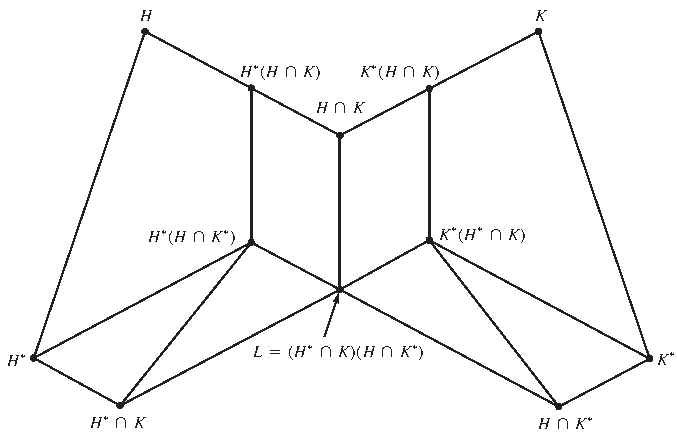
\includegraphics[width=0.929\linewidth,height=.8\textheight,keepaspectratio]{assets/p176_00.pdf}\end{center}
\begin{center}\small\textbf{18.9 Figure}\end{center}
\end{BookFloat}

We now show that \BookInline{H^{\ast }(H\cap K^{\ast })} is a normal subgroup of \BookInline{H^{\ast }(H\cap K).} We let \BookInline{w\in H^{\ast }(H\cap K^{\ast })} and \BookInline{y\in H^{\ast }(H\cap K).} We need to verify that \BookInline{ywy^{- 1}\in H^{\ast }(H\cap K^{\ast }).} By definition\BookInline{,\allowbreak w= h_{1}x} and \BookInline{y\in h_{2}g} for some \BookInline{h_{1},\allowbreak h_{2}\in H^{\ast },\allowbreak x\in H\cap K^{\ast },\allowbreak } and \BookInline{g\in H\cap K.} We write

\begin{center}\begin{adjustbox}{max width=\linewidth}\BookInline{\displaystyle \begin{aligned}ywy^{- 1}&= h_{2}gh_{1}xg^{- 1}h_{2}^{- 1} \\ &= h_{2}(gh_{1}g^{- 1})gxg^{- 1}h_{2}^{- 1} \\ &= h_{2}h_{3}gxg^{- 1}h_{2}^{- 1}\end{aligned}}\end{adjustbox}\end{center}

\noindent for some \BookInline{h_{3}\in H^{\ast }} since \BookInline{H^{\ast }} is a normal subgroup of \BookInline{H.} We note that \BookInline{h_{2}^{- 1}} and \BookInline{h_{2}h_{3}} are both elements of \BookInline{H^{\ast }\leq H^{\ast }(H\cap K^{\ast }).} Furthermore \BookInline{gxg} \BookInline{^ { - 1 } \in K ^ { * }} since \BookInline{g\in K} and \BookInline{K^{\ast }} is a normal subgroup of \BookInline{K.} Also \BookInline{gxg^{- 1}\in H} since both \BookInline{g} and \BookInline{x} are elements of \BookInline{H.} Thus\BookInline{,\allowbreak gxg^{- 1}\in H\cap K^{\ast }\leq K^{\ast }(H\cap K^{\ast }).} So\BookInline{,\allowbreak ywy^{- 1}} is the product of elements in the group \BookInline{H^{\ast }(H\cap K^{\ast }),\allowbreak } which implies that \BookInline{ywy^{- 1}\in H^{\ast }(H\cap K^{\ast }).} Thus we have shown Part 1 of the Theorem.

We use the Second Isomorphism Theorem (16.5) to prove the third part of the Lemma. Let \BookInline{N^{\prime }= H^{\ast }(H\cap K^{\ast })} and \BookInline{H^{\prime }= H\cap K.} So \BookInline{N^{\prime }} is a normal subgroup of \BookInline{H^{\ast }(H\cap K)} and \BookInline{H^{\prime }} is a subgroup of \BookInline{H^{\ast }(H\cup K).} By Lemma \BookInline{16.4N^{\prime }H^{\prime }} is a group and

\begin{center}\begin{adjustbox}{max width=\linewidth}\BookInline{\displaystyle \begin{aligned}N^{\prime }H^{\prime }&= H^{\ast }(H\cap K^{\ast })(H\cap K) \\ &= H^{\ast }(H\cap K).\end{aligned}}\end{adjustbox}\end{center}

\noindent The Second Isomorphism Theorem says that \BookInline{N^{\prime }H^{\prime }/N^{\prime }\simeq H^{\prime }/(H^{\prime }\cap N^{\prime }).} We have

\begin{center}\begin{adjustbox}{max width=\linewidth}\BookInline{\displaystyle N^{\prime }H^{\prime }/N^{\prime }= H^{\ast }(H\cap K)/H^{\ast }(H\cap K^{\ast })}\end{adjustbox}\end{center}

\noindent and

\begin{center}\begin{adjustbox}{max width=\linewidth}\BookInline{\displaystyle H^{\prime }/(H^{\prime }\cap N^{\prime })= (H\cap K)/(H^{\ast }(H\cap K^{\ast })\cap (H\cap K)).}\end{adjustbox}\end{center}

\noindent Exercise 11 in Section 16 shows that

\begin{center}\begin{adjustbox}{max width=\linewidth}\BookInline{\displaystyle H^{\ast }(H\cap K^{\ast })\cap (H\cap K)= (H^{\ast }\cap K)(H\cap K^{\ast }).}\end{adjustbox}\end{center}

\noindent Thus

\begin{center}\begin{adjustbox}{max width=\linewidth}\BookInline{\displaystyle H^{\ast }(H\cap K)/(H^{\ast }(H\cap K^{\ast }))\simeq (H\cap K)/((H^{\ast }\cap K)(H\cap K^{\ast })).}\end{adjustbox}\end{center}

\end{BookBody}

% Source PDF page 177; original printed page 160
\BookSource{177}{160}
\BookNarrativetrue

\begin{BookBody}

By reversing the roles of \BookInline{H} and \BookInline{K(}as well as \BookInline{H^{\ast }} and \BookInline{K^{\ast }),\allowbreak } the proof given above proves Part 2 as well as the other half of Part 3 of the Zassenhaus Lemma\BookInline{.}\BookEnd{\blacklozenge}

\BookLabel{18.11 Theorem} \textbf{(Schreier Theorem)} Two subnormal (normal) series of a group \BookInline{G} have isomorphic refinements.

\BookLabel{\textit{Proof}} Let \BookInline{G} be a group and let

\begin{center}\begin{adjustbox}{max width=\linewidth}\BookInline{\displaystyle \{e\}= H_{0}<H_{1}<H_{2}<\cdots <H_{n}= G(1)}\end{adjustbox}\end{center}

\noindent and

\begin{center}\begin{adjustbox}{max width=\linewidth}\BookInline{\displaystyle \{e\}= K_{0}<K_{1}<K_{2}<\cdots <K_{m}= G(2)}\end{adjustbox}\end{center}

\noindent be two subnormal series for \BookInline{G.} For \BookInline{i} where \BookInline{0\leq i\leq n- 1,\allowbreak } form the chain of groups

\begin{center}\begin{adjustbox}{max width=\linewidth}\BookInline{\displaystyle H_{i}= H_{i}(H_{i+ 1}\cap K_{0})\leq H_{i}(H_{i+ 1}\cap K_{1})\leq \cdots \leq H_{i}(H_{i+ 1}\cap K_{m})= H_{i+ 1}.}\end{adjustbox}\end{center}

\noindent This inserts \BookInline{m- 1} not necessarily distinct groups between \BookInline{H_{i}} and \BookInline{H_{i+ 1}.} If we do this for each \BookInline{i} where \BookInline{0\leq i\leq n- 1} and let \BookInline{H_{i,\allowbreak j}= H_{i}(H_{i+ 1}\cap K_{j}),\allowbreak } then we obtain the chain of groups

\begin{center}\begin{adjustbox}{max width=\linewidth}\BookInline{\displaystyle \begin{aligned}\{e\}&= H_{0,\allowbreak 0}\leq H_{0,\allowbreak 1}\leq H_{0,\allowbreak 2}\leq \cdots \leq H_{0,\allowbreak m- 1}\leq H_{1,\allowbreak 0} \\ &\leq H_{1,\allowbreak 1}\leq H_{1,\allowbreak 2}\leq \cdots \leq H_{1,\allowbreak m- 1}\leq H_{2,\allowbreak 0} \\ &\leq H_{2,\allowbreak 1}\leq H_{2,\allowbreak 2}\leq \cdots \leq H_{2,\allowbreak m- 1}\leq H_{3,\allowbreak 0} \\ &\leq \cdots  \\ &\leq H_{n- 1,\allowbreak 1}\leq H_{n- 1,\allowbreak 2}\leq \cdots \leq H_{n- 1,\allowbreak m- 1}\leq H_{n- 1,\allowbreak m} \\ &= G.(3)\end{aligned}}\end{adjustbox}\end{center}

\noindent This chain (3) contains \BookInline{nm+ 1} not necessarily distinct groups, and \BookInline{H_{i,\allowbreak 0}= H_{i}} for each \BookInline{i.} By the Zassenhaus Lemma, chain (3) is a subnormal chain, that is, each group is normal in the following group. This chain refines the series (1).

In a symmetric fashion, we set \BookInline{K_{j,\allowbreak i}= K_{j}(K_{j+ 1}\cap H_{i})} for \BookInline{0\leq j\leq m- 1} and \BookInline{0\leq i\leq n.} This gives a subnormal chain

\begin{center}\begin{adjustbox}{max width=\linewidth}\BookInline{\displaystyle \begin{aligned}\{e\}&= K_{0,\allowbreak 0}\leq K_{0,\allowbreak 1}\leq K_{0,\allowbreak 2}\leq \cdots \leq K_{0,\allowbreak n- 1}\leq K_{1,\allowbreak 0} \\ &\leq K_{1,\allowbreak 1}\leq K_{1,\allowbreak 2}\leq \cdots \leq K_{1,\allowbreak n- 1}\leq K_{2,\allowbreak 0} \\ &\leq K_{2,\allowbreak 1}\leq K_{2,\allowbreak 2}\leq \cdots \leq K_{2,\allowbreak n- 1}\leq K_{3,\allowbreak 0} \\ &\leq \cdots  \\ &\leq K_{m- 1,\allowbreak 1}\leq K_{m- 1,\allowbreak 2}\leq \cdots \leq K_{m- 1,\allowbreak n- 1}\leq K_{m- 1,\allowbreak n} \\ &= G.(4)\end{aligned}}\end{adjustbox}\end{center}

\noindent This chain (4) contains \BookInline{mn+ 1} not necessarily distinct groups, and \BookInline{K_{j,\allowbreak 0}= K_{j}} for each \BookInline{j.} This chain refines the series (2).

By the Zassenhaus Lemma 18.10, we have

\begin{center}\begin{adjustbox}{max width=\linewidth}\BookInline{\displaystyle H_{i}(H_{i+ 1}\cap K_{j+ 1})/H_{i}(H_{i+ 1}\cap K_{j})\simeq K_{j}(K_{j+ 1}\cap H_{i+ 1})/K_{j}(K_{j+ 1}\cap H_{i}),\allowbreak }\end{adjustbox}\end{center}

\noindent or

\begin{center}\begin{adjustbox}{max width=\linewidth}\BookInline{\displaystyle H_{i,\allowbreak j+ 1}/H_{i,\allowbreak j}\simeq K_{j,\allowbreak i+ 1}/K_{j,\allowbreak i}(5)}\end{adjustbox}\end{center}

\noindent for \BookInline{0\leq i\leq n- 1} and \BookInline{0\leq j\leq m- 1.} The isomorphisms of relation (5) give a one-toone correspondence of isomorphic factor groups between the subnormal chains (3) and (4). To verify this correspondence, note that \BookInline{H_{i,\allowbreak 0}= H_{i}} and \BookInline{H_{i,\allowbreak m}= H_{i+ 1},\allowbreak } while \BookInline{K_{j,\allowbreak 0}= K_{j}} and \BookInline{K_{j,\allowbreak n}= K_{j+ 1}.} Each chain in (3) and (4) contains a rectangular array of \BookInline{mn} symbols \BookInline{\leq.} Each \BookInline{\leq } gives rise to a factor group. The factor groups arising from the \BookInline{r}th\textit{ row} of \BookInline{\leq }’s 
% Source PDF page 178; original printed page 161
\BookSource{178}{161}
in chain (3) correspond to the factor groups arising from the \BookInline{r}th\textit{ column} of \BookInline{\leq }’s in chain (4). Deleting repeated groups from the chains in (3) and (4), we obtain subnormal series of distinct groups that are isomorphic refinements of chains (1) and (2). This establishes the theorem for subnormal series.

\end{BookBody}

\BookNarrativetrue

\begin{BookBody}

For normal series, where all \BookInline{H_{i}} and \BookInline{K_{j}} are normal in \BookInline{G,\allowbreak } we merely observe that all the groups \BookInline{H_{i,\allowbreak j}} and \BookInline{K_{j,\allowbreak i}} formed above are also normal in \BookInline{G,\allowbreak } so the same proof applies. This normality of \BookInline{H_{i,\allowbreak j}} and \BookInline{K_{j,\allowbreak i}} follows at once from the second assertion in Lemma 16.4 and from the fact that intersections of normal subgroups of a group yield normal subgroups\BookInline{.}\BookEnd{\blacklozenge}

\BookTextHeading{\textbf{The Jordan–Ho¨ lder Theorem}  }

\noindent We now come to the real meat of the theory.

\BookLabel{18.12 Definition} A subnormal series \BookInline{\{H_{i}\}} of a group \BookInline{G} is a\textbf{ composition series} if all the factor groups \BookInline{H_{i+ 1}/H_{i}} are simple. A normal series \BookInline{\{H_{i}\}} of \BookInline{G} is a\textbf{ principal} or\textbf{ chief series} if all the factor groups \BookInline{H_{i+ 1}/H_{i}} are simple\BookInline{.}\BookEnd{\blacksquare}

Note that for abelian groups the concepts of composition and principal series coincide. Also, since every normal series is subnormal, every principal series is a composition series for any group, abelian or not.

\BookLabel{18.13 Example} We claim that \BookInline{\mathbb{Z}} has no composition (and also no principal) series. For if

\begin{center}\begin{adjustbox}{max width=\linewidth}\BookInline{\displaystyle \{0\}= H_{0}<H_{1}<\cdots <H_{n- 1}<H_{n}= \mathbb{Z}}\end{adjustbox}\end{center}

\noindent is a subnormal series\BookInline{,\allowbreak H_{1}} must be of the form \BookInline{r\mathbb{Z}} for some \BookInline{r\in \mathbb{Z}^{+ }.} But then \BookInline{H_{1}/H_{0}} is isomorphic to \BookInline{r\mathbb{Z},\allowbreak } which is infinite cyclic with many nontrivial proper normal subgroups, for example\BookInline{,\allowbreak 2r\mathbb{Z}.} Thus \BookInline{\mathbb{Z}} has no composition (and also no principal) series. \BookEnd{\blacktriangle}

\BookLabel{18.14 Example} The series

\begin{center}\begin{adjustbox}{max width=\linewidth}\BookInline{\displaystyle \{e\}<A_{n}<S_{n}}\end{adjustbox}\end{center}

\noindent for \BookInline{n\geq 5} is a composition series (and also a principal series) of \BookInline{S_{n},\allowbreak } because \BookInline{A_{n}/\{e\}} is isomorphic to \BookInline{A_{n},\allowbreak } which is simple for \BookInline{n\geq 5,\allowbreak } and \BookInline{S_{n}/A_{n}} is isomorphic to \BookInline{\mathbb{Z}_{2},\allowbreak } which is simple. Likewise, the two series given in Example 18.7 are composition series (and also principal series) of \BookInline{\mathbb{Z}_{15}.} They are isomorphic, as shown in that example. This illustrates our main theorem, which will be stated shortly\BookInline{.}\BookEnd{\blacktriangle}

Observe that by Theorem \BookInline{13.20,\allowbreak H_{i+ 1}/H_{i}} is simple if and only if \BookInline{H_{i}} is a maximal normal subgroup of \BookInline{H_{i+ 1}.} Thus for a composition series, each \BookInline{H_{i}} must be a maximal normal subgroup of \BookInline{H_{i+ 1}.} \textit{To form} \BookInline{a} \textit{composition series of} \BookInline{a} \textit{group} \BookInline{G,\allowbreak } \textit{we just} \BookInline{hunt} \textit{for} \BookInline{a} \textit{maximal normal subgroup} \BookInline{H_{n- 1}} \textit{of} \BookInline{G,\allowbreak } \textit{then for} \BookInline{a} \textit{maximal normal subgroup} \BookInline{H_{n- 2}} \textit{of} \BookInline{H_{n- 1},\allowbreak } \textit{and so on}.\textit{ If this process terminates in} \BookInline{a} \textit{finite number of steps, we have} \BookInline{a} \textit{composition series}. Note that by Theorem 13.20, a composition series cannot have any further refinement.\textit{ To form} \BookInline{a} \textit{principal series, we have to} \BookInline{hunt} \textit{for} \BookInline{a} \textit{maximal normal} \textit{subgroup} \BookInline{H_{n- 1}} \textit{of} \BookInline{G,\allowbreak } \textit{then for} \BookInline{a} \textit{maximal normal subgroup} \BookInline{H_{n- 2}} \textit{of} \BookInline{H_{n- 1}} \textit{that is also} \textit{normal in} \BookInline{G,\allowbreak } \textit{and so on}. The main theorem is as follows.

\BookLabel{18.15 Theorem} \textbf{(Jordan–Ho¨lder Theorem)} Any two composition (principal) series of a group \BookInline{G} are isomorphic.

\BookLabel{\textit{Proof}} Let \BookInline{\{H_{i}\}} and \BookInline{\{K_{i}\}} be two composition (principal) series of \BookInline{G.} By Theorem 18.11, they have isomorphic refinements. But since all factor groups are already simple,

\end{BookBody}

% Source PDF page 179; original printed page 162
\BookSource{179}{162}
\BookNarrativetrue

\begin{BookBody}

\noindent Theorem 13.20 shows that neither series has any further refinement. Thus \BookInline{\{H_{i}\}} and \BookInline{\{K_{i}\}} must already be isomorphic\BookInline{.}\BookEnd{\blacklozenge}

For a finite group, we should regard a composition series as a type of factorization of the group into simple factor groups, analogous to the factorization of a positive integer into primes. In both cases, the factorization is unique, up to the order of the factors.

\BookLabel{18.16 Example} We illustrate the analogy between factoring integers and composition series with an example. Let \BookInline{n\in \mathbb{Z}^{+ }.} We factor \BookInline{n} into its prime factors \BookInline{n= p_{1}p_{2}p_{3}...p_{k},\allowbreak } where the prime factors may be repeated and they are in any order. The series

\begin{center}\begin{adjustbox}{max width=\linewidth}\BookInline{\displaystyle \{0\}<\langle p_{1}p_{2}p_{3}\cdots p_{k- 1}\rangle <\langle p_{1}p_{2}p_{3}\cdots p_{k- 2}\rangle <\langle p_{1}p_{2}p_{3}\cdots p_{k- 3}\rangle <\cdots <\langle p_{1}\rangle <\mathbb{Z}_{n}}\end{adjustbox}\end{center}

\noindent is a composition series since the factor groups are isomorphic with \BookInline{\mathbb{Z}_{p_{k}},\allowbreak \mathbb{Z}_{p_{k- 1}},\allowbreak \mathbb{Z}_{p_{k- 2}},\allowbreak...}, \BookInline{\mathbb{Z}_{p_{1}}}, which are all simple. For each choice of ordering the prime numbers \BookInline{p_{1},\allowbreak p_{2},\allowbreak...,\allowbreak p_{k}} we get a different composition series, but they are all isomorphic since the factor groups are \BookInline{\mathbb{Z}_{p_{1}},\allowbreak \mathbb{Z}_{p_{2}},\allowbreak...,\allowbreak \mathbb{Z}_{p_{k}}} in some order\BookInline{.}\BookEnd{\blacktriangle}

\BookTextHeading{\ensuremath{\blacksquare} \textbf{HISTORICAL NOTE}  }

\noindent This first appearance of what became the Jordan–Ho¨lder theorem occurred in 1869 in a commentary on the work of Galois by the brilliant French algebraist Camille Jordan (1838– 1922). The context of its appearance is the study of permutation groups associated with the roots of polynomial equations. Jordan asserted that even though the sequence of normal subgroups \BookInline{G,\allowbreak I,\allowbreak J,\allowbreak \cdots } of the group of the equation is not necessarily unique, nevertheless the sequence of indices of this composition series is unique. Jordan gave a proof in his monumental 1870\textit{ Treatise on Substitutions and Algebraic} \textit{Equations}. This latter work, though restricted to what we now call permutation groups, remained the standard treatise on group theory for many years.

The Ho¨lder part of the theorem, that the sequence of factor groups in a composition series is unique up to order, was due to Otto Ho¨lder (1859– 1937), who played a very important role in the development of group theory once the completely abstract definition of a group had been given. Among his other contributions, he gave the first abstract definition of a “factor group” and determined the structure of all finite groups of square-free order.

\BookLabel{18.17 Theorem} If \BookInline{G} has a composition (principal) series, and if \BookInline{N} is a proper normal subgroup of \BookInline{G,\allowbreak } then there exists a composition (principal) series containing \BookInline{N.}

\BookLabel{\textit{Proof}} The series

\begin{center}\begin{adjustbox}{max width=\linewidth}\BookInline{\displaystyle \{e\}<N<G}\end{adjustbox}\end{center}

\noindent is both a subnormal and a normal series. Since \BookInline{G} has a composition series \BookInline{\{H_{i}\},\allowbreak } then by Theorem 18.11 there is a refinement of \BookInline{\{e\}<N<G} to a subnormal series isomorphic to a refinement of \BookInline{\{H_{i}\}.} But as a composition series\BookInline{,\allowbreak \{H_{i}\}} can have no further refinement. Thus \BookInline{\{e\}<N<G} can be refined to a subnormal series all of whose factor groups are simple, that is, to a composition series. A similar argument holds if we start with a principal series \BookInline{\{K_{j}\}} of \BookInline{G.}\BookEnd{\blacklozenge}

\BookLabel{18.18 Example} A composition (and also a principal) series of \BookInline{\mathbb{Z}_{4}\times \mathbb{Z}_{9}} containing \BookInline{\langle (0,\allowbreak 1)\rangle } is

\begin{center}\begin{adjustbox}{max width=\linewidth}\BookInline{\displaystyle \{(0,\allowbreak 0)\}<\langle (0,\allowbreak 3)\rangle <\langle (0,\allowbreak 1)\rangle <\langle 2\rangle \times \langle 1\rangle <\langle 1\rangle \times \langle 1\rangle = \mathbb{Z}_{4}\times \mathbb{Z}_{9}.}\end{adjustbox}\end{center} \BookEnd{\blacktriangle}

\end{BookBody}

% Source PDF page 180; original printed page 163
\BookSource{180}{163}
\BookNarrativetrue

\begin{BookBody}

The next definition is basic to the characterization of those polynomial equations whose solutions can be expressed in terms of radicals.

\BookLabel{18.19 Definition} A group \BookInline{G} is\textbf{ solvable} if it has a composition series \BookInline{\{H_{i}\}} such that all factor groups \BookInline{H_{i+ 1}/H_{i}} are abelian\BookInline{.}\BookEnd{\blacksquare}

By the Jordan–Ho¨lder theorem, we see that for a solvable group,\textit{ every} composition series \BookInline{\{H_{i}\}} must have abelian factor groups \BookInline{H_{i+ 1}/H_{i}.}

\BookLabel{18.20 Example} The group \BookInline{S_{3}} is solvable, because the composition series

\begin{center}\begin{adjustbox}{max width=\linewidth}\BookInline{\displaystyle \{e\}<A_{3}<S_{3}}\end{adjustbox}\end{center}

\noindent has factor groups isomorphic to \BookInline{\mathbb{Z}_{3}} and \BookInline{\mathbb{Z}_{2},\allowbreak } which are abelian. The group \BookInline{S_{5}} is not solvable, for since \BookInline{A_{5}} is simple, the series

\begin{center}\begin{adjustbox}{max width=\linewidth}\BookInline{\displaystyle \{e\}<A_{5}<S_{5}}\end{adjustbox}\end{center}

\noindent is a composition series, and \BookInline{A_{5}/\{e\},\allowbreak } which is isomorphic to \BookInline{A_{5},\allowbreak } is not abelian.\textit{ This group} \BookInline{A_{5}} \textit{of order} 60\textit{ can be shown to be the smallest group that is not solvable}. This fact is closely connected with the fact that a polynomial equation of degree 5 is not in general solvable by radicals, but a polynomial equation of degree \BookInline{\leq 4} is\BookInline{.}\BookEnd{\blacktriangle}

\BookTextHeading{\textbf{The Ascending Central Series}  }

\noindent We mention one subnormal series for a group \BookInline{G} that can be formed using centers of groups. Recall from Section 13 that the center \BookInline{Z(G)} of a group \BookInline{G} is defined by

\begin{center}\begin{adjustbox}{max width=\linewidth}\BookInline{\displaystyle Z(G)= \{z\in G\mid zg= gz\;\text{for all}\;g\in G\},\allowbreak }\end{adjustbox}\end{center}

\noindent and that \BookInline{Z(G)} is a normal subgroup of \BookInline{G.} If we have the table for a finite group \BookInline{G,\allowbreak } it is easy to find the center. An element \BookInline{a} is in the center of \BookInline{G} if and only if the row with header \BookInline{a} and the column with header \BookInline{a} list the elements of \BookInline{G} in the same order.

Now let \BookInline{G} be a group, and let \BookInline{Z(G)} be the center of \BookInline{G.} Since \BookInline{Z(G)} is normal in \BookInline{G,\allowbreak } we can form the factor group \BookInline{G/Z(G)} and find the center \BookInline{Z(G/Z(G))} of this factor group. Since \BookInline{Z(G/Z(G))} is normal in \BookInline{G/Z(G),\allowbreak } if \BookInline{\gamma:G\to G/Z(G)} is the canonical map, then by Theorem \BookInline{13.18,\allowbreak \gamma ^{- 1}[Z(G/Z(G))]} is a normal subgroup \BookInline{Z_{1}(G)} of \BookInline{G.} We can then form the factor group \BookInline{G/Z_{1}(G)} and find its center, take \BookInline{(\gamma _{1})^{- 1}} of it to get \BookInline{Z_{2}(G),\allowbreak } and so on.

\BookLabel{18.21 Definition} The series

\begin{center}\begin{adjustbox}{max width=\linewidth}\BookInline{\displaystyle \{e\}\leq Z(G)\leq Z_{1}(G)\leq Z_{2}(G)\leq \cdots}\end{adjustbox}\end{center}

\noindent described in the preceding discussion is the\textbf{ ascending central series of the group} \BookInline{G.} \BookEnd{\blacksquare}

\BookLabel{18.22 Example} For \BookInline{n\geq 3,\allowbreak } the center of \BookInline{S_{n}} is just the identity \BookInline{\iota.} Thus the ascending central series of \BookInline{S_{n}} is

\begin{center}\begin{adjustbox}{max width=\linewidth}\BookInline{\displaystyle \{\iota \}\leq \{\iota \}\leq \{\iota \}\leq ....}\end{adjustbox}\end{center}

\noindent The center of the dihedral group \BookInline{D_{4}} is \BookInline{\{\iota,\allowbreak \rho ^{2}\}.} The factor group \BookInline{D_{4}/\{\iota,\allowbreak \rho ^{2}\}} has order 4, and each element has order 1 or 2, so \BookInline{D_{4}/\{\iota,\allowbreak \rho ^{2}\}} is isomorphic with the Klein 4-group, which is abelian. Therefore the center of \BookInline{D_{4}/\{\iota,\allowbreak \rho ^{2}\}} is the whole group, and the central series for \BookInline{D_{4}} is

\begin{center}\begin{adjustbox}{max width=\linewidth}\BookInline{\displaystyle \{\iota \}\leq \{\iota ,\allowbreak \rho ^{2}\}\leq D_{4}\leq D_{4}\leq D_{4}\leq ....}\end{adjustbox}\end{center} \BookEnd{\blacktriangle}

\end{BookBody}

% Source PDF page 181; original printed page 164
\BookSource{181}{164}
\BookNarrativefalse

\begin{BookBody}

\BookExerciseTitle{18}

\BookTextHeading{\textbf{Computations}}

\noindent In Exercises 1 through 5, give isomorphic refinements of the two series.

\BookExercise{1.}{\BookInline{\{0\}<10\mathbb{Z}<\mathbb{Z}} and \BookInline{\{0\}<25\mathbb{Z}<\mathbb{Z}}}

\BookExercise{2.}{\BookInline{\{0\}<60\mathbb{Z}<20\mathbb{Z}<\mathbb{Z}} and \BookInline{\{0\}<245\mathbb{Z}<49\mathbb{Z}<\mathbb{Z}}}

\BookExercise{3.}{\BookInline{\{0\}<\langle 9\rangle <\mathbb{Z}_{54}} and \BookInline{\{0\}<\langle 2\rangle <\mathbb{Z}_{54}}}

\BookExercise{4.}{\BookInline{\{0\}<\langle 9\rangle <\langle 3\rangle <\mathbb{Z}_{72}} and \BookInline{\{0\}<\langle 36\rangle <\langle 12\rangle <\mathbb{Z}_{72}}}

\BookExercise{5.}{\BookInline{\{(0,\allowbreak 0)\}<(60\mathbb{Z})\times \mathbb{Z}<(10\mathbb{Z})\times \mathbb{Z}<\mathbb{Z}\times \mathbb{Z}} and \BookInline{\{(0,\allowbreak 0)\}<\mathbb{Z}\times (80\mathbb{Z})<\mathbb{Z}\times (20\mathbb{Z})<\mathbb{Z}\times \mathbb{Z}}}

\BookExercise{6.}{Find all composition series of \BookInline{\mathbb{Z}_{90}} and show that they are isomorphic.}

\BookExercise{7.}{Find all composition series of \BookInline{\mathbb{Z}_{48}} and show that they are isomorphic.}

\BookExercise{8.}{Find all composition series of \BookInline{\mathbb{Z}_{5}\times \mathbb{Z}_{5}.}}

\BookExercise{9.}{Find all composition series of \BookInline{S_{3}\times \mathbb{Z}_{2}.}}

\BookExercise{10.}{Find all composition series of \BookInline{\mathbb{Z}_{2}\times \mathbb{Z}_{5}\times \mathbb{Z}_{7}.}}

\BookExercise{11.}{Find the center of \BookInline{S_{3}\times \mathbb{Z}_{4}.}}

\BookExercise{12.}{Find the center of \BookInline{S_{3}\times D_{4}.}}

\BookExercise{13.}{Find the ascending central series of \BookInline{S_{3}\times \mathbb{Z}_{4}.}}

\BookExercise{14.}{Find the ascending central series of \BookInline{S_{3}\times D_{4}.}}

\BookTextHeading{\textbf{Concepts}}

\noindent In Exercises 15 and 16, correct the definition of the italicized term without reference to the text, if correction is needed, so that it is in a form acceptable for publication.

\BookExercise{15.}{A\textit{ composition series} of a group \BookInline{G} is a finite sequence}

\begin{center}\begin{adjustbox}{max width=\linewidth}\BookInline{\displaystyle \{e\}= H_{0}<H_{1}<H_{2}<\cdots <H_{n- 1}<H_{n}= G}\end{adjustbox}\end{center}

of subgroups of \BookInline{G} such that \BookInline{H_{i}} is a maximal normal subgroup of \BookInline{H_{i+ 1}} for \BookInline{i= 0,\allowbreak 1,\allowbreak 2,\allowbreak \cdots,\allowbreak n- 1.}

\BookExercise{16.}{A\textit{ solvable group} is one that has a composition series of abelian groups.}

\BookExercise{17.}{Determine whether each of the following is true or false.}

\BookExercise{a.}{Every normal series is also subnormal.}

\BookExercise{b.}{Every subnormal series is also normal.}

\BookExercise{c.}{Every principal series is a composition series.}

\BookExercise{d.}{Every composition series is a principal series.}

\BookExercise{e.}{Every abelian group has exactly one composition series.}

\BookExercise{f.}{Every finite group has a composition series.}

\BookExercise{g.}{A group is solvable if and only if it has a composition series with simple factor groups.}

\BookExercise{h.}{\textbf{h}\BookInline{.S_{7}} is a solvable group.}

\BookExercise{i.}{The Jordan–Ho¨lder theorem has some similarity with the Fundamental Theorem of Arithmetic, which states that every positive integer greater than 1 can be factored into a product of primes uniquely up to order.}

\BookExercise{j.}{Every finite group of prime order is solvable.}

\BookExercise{18.}{Find a composition series of \BookInline{S_{3}\times S_{3}.} Is \BookInline{S_{3}\times S_{3}} solvable?}

\BookExercise{19.}{Is the dihedral group \BookInline{D_{4}} solvable?}

\BookExercise{20.}{Let \BookInline{G} be \BookInline{\mathbb{Z}_{36}.} Refer to the proof of Theorem 18.11. Let the subnormal series (1) be}

\begin{center}\begin{adjustbox}{max width=\linewidth}\BookInline{\displaystyle \{0\}<\langle 12\rangle <\langle 3\rangle <\mathbb{Z}_{36}}\end{adjustbox}\end{center}

and let the subnormal series (2) be

\begin{center}\begin{adjustbox}{max width=\linewidth}\BookInline{\displaystyle \{0\}<\langle 18\rangle <\mathbb{Z}_{36}.}\end{adjustbox}\end{center}

\end{BookBody}

% Source PDF page 182; original printed page 165
\BookSource{182}{165}
\BookNarrativefalse

\begin{BookBody}

Find chains (3) and (4) and exhibit the isomorphic factor groups as described in the proof. Write chains (3) and (4) in the rectangular array shown in the text.

\BookExercise{21.}{Repeat Exercise 20 for the group \BookInline{\mathbb{Z}_{24}} with the subnormal series (1)}

\begin{center}\begin{adjustbox}{max width=\linewidth}\BookInline{\displaystyle \{0\}<\langle 12\rangle <\langle 4\rangle <\mathbb{Z}_{24}}\end{adjustbox}\end{center}

and (2)

\begin{center}\begin{adjustbox}{max width=\linewidth}\BookInline{\displaystyle \{0\}<\langle 6\rangle <\langle 3\rangle <\mathbb{Z}_{24}.}\end{adjustbox}\end{center}

\BookTextHeading{\textbf{Theory}}

\BookExercise{22.}{Let \BookInline{H^{\ast },\allowbreak H,\allowbreak } and \BookInline{K} be subgroups of \BookInline{G} with \BookInline{H^{\ast }} normal in \BookInline{H.} Show that \BookInline{H^{\ast }\cap K} is normal in \BookInline{H\cap K.}}

\BookExercise{23.}{Show that if}

\begin{center}\begin{adjustbox}{max width=\linewidth}\BookInline{\displaystyle H_{0}= \{e\}<H_{1}<H_{2}<\cdots <H_{n}= G}\end{adjustbox}\end{center}

is a subnormal (normal) series for a group \BookInline{G,\allowbreak } and if \BookInline{H_{i+ 1}/H_{i}} is of finite order \BookInline{s_{i+ 1},\allowbreak } then \BookInline{G} is of finite order \BookInline{s_{1}s_{2}\cdots s_{n}.}

\BookExercise{24.}{Show that an infinite abelian group can have no composition series. [\textit{Hint:} Use Exercise 23, together with the fact that an infinite abelian group always has a proper nontrivial subgroup.]}

\BookExercise{25.}{Show that a finite direct product of solvable groups is solvable.}

\BookExercise{26.}{Show that if \BookInline{H\unlhd G} is a normal subgroup\BookInline{,\allowbreak H} is solvable, and \BookInline{G/H} is solvable, then \BookInline{G} is solvable.}

\BookExercise{27.}{Show that for \BookInline{n\geq 3,\allowbreak D_{n}} is solvable.}

\BookExercise{28.}{Show that a subgroup \BookInline{K} of a solvable group \BookInline{G} is solvable. [\textit{Hint:} Let \BookInline{H_{0}= \{e\}<H_{1}<\cdots <H_{n}= G} be a composition series for \BookInline{G.} Show that the distinct groups among \BookInline{K\cap H_{i}} for \BookInline{i= 0,\allowbreak \cdots,\allowbreak n} form a composition series for \BookInline{K.} Observe that}

\begin{center}\begin{adjustbox}{max width=\linewidth}\BookInline{\displaystyle (K\cap H_{i})/(K\cap H_{i- 1})\simeq [H_{i- 1}(K\cap H_{i})]/[H_{i- 1}],\allowbreak }\end{adjustbox}\end{center}

by Theorem 16.5, with \BookInline{H= K\cap H_{i}} and \BookInline{N= H_{i- 1},\allowbreak } and that \BookInline{H_{i- 1}(K\cap H_{i})\leq H_{i}.]}

\BookExercise{29.}{Let \BookInline{H_{0}= \{e\}<H_{1}<\cdots <H_{n}= G} be a composition series for a group \BookInline{G.} Let \BookInline{N} be a normal subgroup of \BookInline{G,\allowbreak } and suppose that \BookInline{N} is a simple group. Show that the distinct groups among \BookInline{H_{0},\allowbreak H_{i}N} for \BookInline{i= 0,\allowbreak \cdots,\allowbreak n} also form a composition series for \BookInline{G.[}\textit{Hint}\BookInline{:H_{i}N} is a group by Lemma 16.4. Show that \BookInline{H_{i- 1}N} is normal in \BookInline{H_{i}N.} By Theorem 16.5}

\begin{center}\begin{adjustbox}{max width=\linewidth}\BookInline{\displaystyle (H_{i}N)/(H_{i- 1}N)\simeq H_{i}/[H_{i}\cap (H_{i- 1}N)],\allowbreak }\end{adjustbox}\end{center}

and the latter group is isomorphic to

\begin{center}\begin{adjustbox}{max width=\linewidth}\BookInline{\displaystyle [H_{i}/H_{i- 1}]/[(H_{i}\cap (H_{i- 1}N))/H_{i- 1}],\allowbreak }\end{adjustbox}\end{center}

by Theorem 16.8. But \BookInline{H_{i}/H_{i- 1}} is simple.]

\BookExercise{30.}{Let \BookInline{G} be a group, and let \BookInline{H_{0}= \{e\}<H_{1}<\cdots <H_{n}= G} be a composition series for \BookInline{G.} Let \BookInline{N} be a normal subgroup of \BookInline{G,\allowbreak } and let \BookInline{\gamma:G\to G/N} be the canonical map. Show that the distinct groups among \BookInline{\gamma [H_{i}]} for \BookInline{i= 0,\allowbreak \cdots,\allowbreak n,\allowbreak } form a composition series for \BookInline{G/N.[}\textit{Hint:} Observe that the map}

\begin{center}\begin{adjustbox}{max width=\linewidth}\BookInline{\displaystyle \psi :H_{i}N\to \gamma [H_{i}]/\gamma [H_{i- 1}]}\end{adjustbox}\end{center}

defined by

\begin{center}\begin{adjustbox}{max width=\linewidth}\BookInline{\displaystyle \psi (h_{i}n)= \gamma (h_{i}n)\gamma [H_{i- 1}]}\end{adjustbox}\end{center}

is a homomorphism with kernel \BookInline{H_{i- 1}N.} By Theorem 16.2.

\begin{center}\begin{adjustbox}{max width=\linewidth}\BookInline{\displaystyle \gamma [H_{i}]/\gamma [H_{i- 1}]\simeq (H_{i}N)/(H_{i- 1}N).}\end{adjustbox}\end{center}

Proceed via Theorem 16.5, as shown in the hint for Exercise 29.]

\BookExercise{31.}{Prove that a homomorphic image of a solvable group is solvable. [\textit{Hint:} Apply Exercise 30 to get a composition series for the homomorphic image. The hints for Exercises 29 and 30 then show how the factor groups of this composition series in the image look.]}

\BookExercise{32.}{Prove that a finite \BookInline{p-}group is solvable.}

\end{BookBody}
\ifdefined\BookMaster\let\BookFinish\relax\else\def\BookFinish{\end{document}}\fi\BookFinish
